\documentclass[11pt]{lecture}

% \usepackage{chronology} %% for timeline
\def\fullsize{0.55\textwidth}

\usepackage{xcolor}
\hypersetup{
    colorlinks,
    linkcolor={red!50!black},
    citecolor={blue!50!black},
    urlcolor={blue!80!black}
}

\usepackage{booktabs}
\usepackage{multirow}

\begin{document}

\course{CS 6210/CS 4210 ADVANCED OPERATING SYSTEMS}
\title{Distributed Shared Memory (Part II)}%\footnotemark[1]\footnotemark[2]
\semester{Fall 2017}
\instructor{Prof. Umakishore Ramachandran}
\author{Long Gong}
\footnotetext[1]{All the figures in this scribe are directly from or modified from the lecture 
slides provided by Prof. Umakishore Ramachandran.}
\maketitle

\section{Overview}\label{sec: overview}

In this lecture, we will cover the details of the multiple-writer coherence protocol, and some details 
for the implementations of LRC with multi-writer coherence protocol


\section{LRC with Multi-Writer Coherence Protocol}\label{sec: lrc-mwcp}

In the previous lecture, we have talked about the single-writer multiple-reader protocol for Lazy RC (LRC). 
The false sharing problem associated it brings us the new protocol, which is called multiple-writer 
protocol. The idea is we want to maintain the coherence information still at the granularity
of pages. Because that is the granularity at which the operating system operates and therefore the DSM 
can be integrated with the operating system. But at the same time, we want to allow multiple writers to be able to 
same page recognizing that application programmer may have packed lots of different data structures 
within the same page. So we are going to see how the multiple-writer coherence protocol 
works and in particular we are going to use that in concert with lazy RC. The background of what is going to describe 
is covered in the TreadMarks paper~\cite{Amza1996DSM}. 


\begin{figure}[!htbp]
\centering 
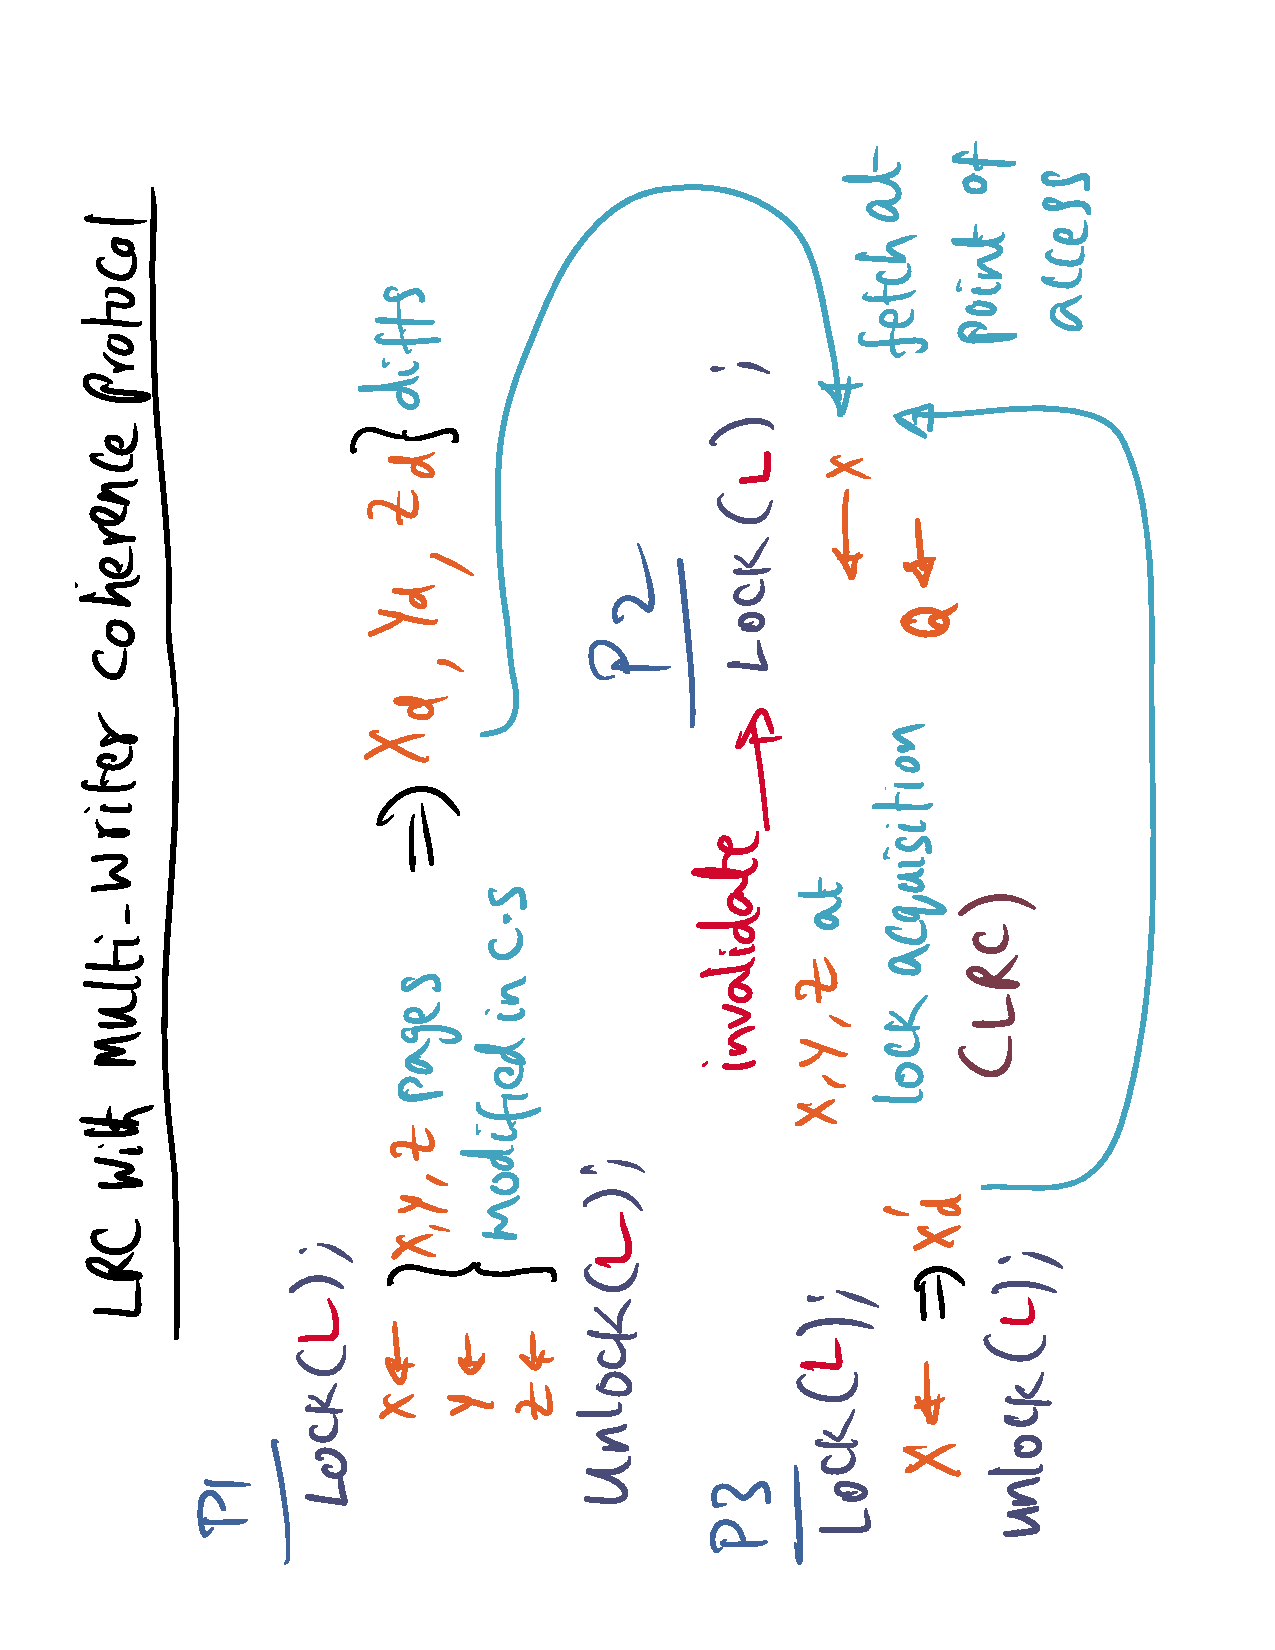
\includegraphics[width=\fullsize, angle=-90]{Figures/mwcp}
\caption{LRC with multiple-writer coherence protocol.}\label{fig: mwcp}
\end{figure}

As shown in~\autoref{fig: mwcp}, a process of $P1$ acquires a lock and makes modifications. Note that, the notations 
{\code x, y, z} stand for three different pages. And by modifications, we mean the modification to the 
data structures that are contained in these pages. Therefore, pages {\code x, y, z} are those pages 
that are being modified within the critical section when processor $P1$ executes the piece of code 
shown in~\autoref{fig: mwcp}. Note that, the operating system has no knowledge of the association the lock 
{\code L} and the pages that are being modified. All it knows is that within the critical section, 
these pages ({\it i.e.,} pages {\code x, y, z}) are the pages that were modified. That is what the operating 
system knows. What we are going to do is we are going to create a {\it diff} of the changes that 
were made to the pages {\code x, y, z}. We know at the beginning of this critical section, 
what the contents of the pages {\code x, y, z} are and at the end of this critical section, we 
are going to find out what is the difference (or changes) that has been made and compute the 
``diffs'' between the original pages and modified ones, {\it i.e.,} $x_d, y_d, z_d$. 

So the next time the same lock {\code L} is acquired by some of the process of $P2$. We are going to first invalidate 
the pages were modified by the previous lock holder. Note that, although the LRC does not know these ``diffs'', it 
knows the association between the lock and the pages that are modified within the critical section governed 
by this lock. So when $P2$ makes this lock acquisition, the DSM is going to first invalidate: If copies 
of pages {\code x, y, z} are locally resident in the process of $P2$, then the DSM software is 
going to invalidate those copies at the point of lock acquisition. That is consistent with the lazy 
release consistency model. So once we have invalidated these pages, then we can allow $P2$ to get the lock 
and start its critical section. Once it is in the critical section, it can do whatever it wants but if 
it tries to access some modified page, say page {\code x}. The DSM software will get into action: It will first 
get the original copy of the page from its owner, and get the ``diffs'' from the previous holder 
of the lock to create the current version of the page. 

What if, prior to $P2$ getting its lock, another processor (say $P3$) also used the same lock. 
So when $P3$ executes its critical section, it modified the page {\code x} again, and 
it creates its own ``diffs'', $x'_d$. Because all of these locks are the same, the DSM software 
knows that now there are two ``diffs'' associated with this lock {\code L}: One ``diffs'' is 
with the processor $P1$, and another is residing with processor $P3$. Therefore, when processor 
$P2$ tries to access page {\code x}, the DSM software has not only to get the ``diffs'' from 
$P1$, but it also needs the ``diffs'' from $P3$, and apply it to the original, pristine 
version of the page that is with the owner of the page. So that it can create the current version 
of the page. And you can extend this to any number of processors that may have made modifications 
under the provision of the lock {\code L}. All of those ``diffs'' are going to be applied in order for the 
processors of $P2$ to access the page as the current page. If after accessing the page {\code x} 
and during its execution $P2$ touches, say page {\code z}, in its critical section. Once again, the DSM software 
will get all the ``diffs'' from previous holders of the same lock, and apply the ``diffs'' to the 
original copy of page {\code z}. So you can see that even though the invalidation was done 
right at the beginning of a critical section, we are procrastinating getting the 
``diffs'' until the point of access. Note that, it is possible that $P2$, as part of its execution 
of its critical section, modifies another page, say page {\code w}, different from {\code x, y, z}. 
So now the DSM software knows that this particular lock ({\it i.e.,} lock {\code L}) is associated 
not just with pages {\code x, y} and {\code z}, but is is also associated with page {\code w}. So 
future lock acquisition for {\code L} will result in invalidating {\code x, y, z} and {\code w}, because 
all of those pages may have been modified. And the next critical section wants to access this lock {\code L} 
has to get the current versions of all the pages that were ever associated with {\code L}. 

\begin{figure}[!htbp]
\centering 
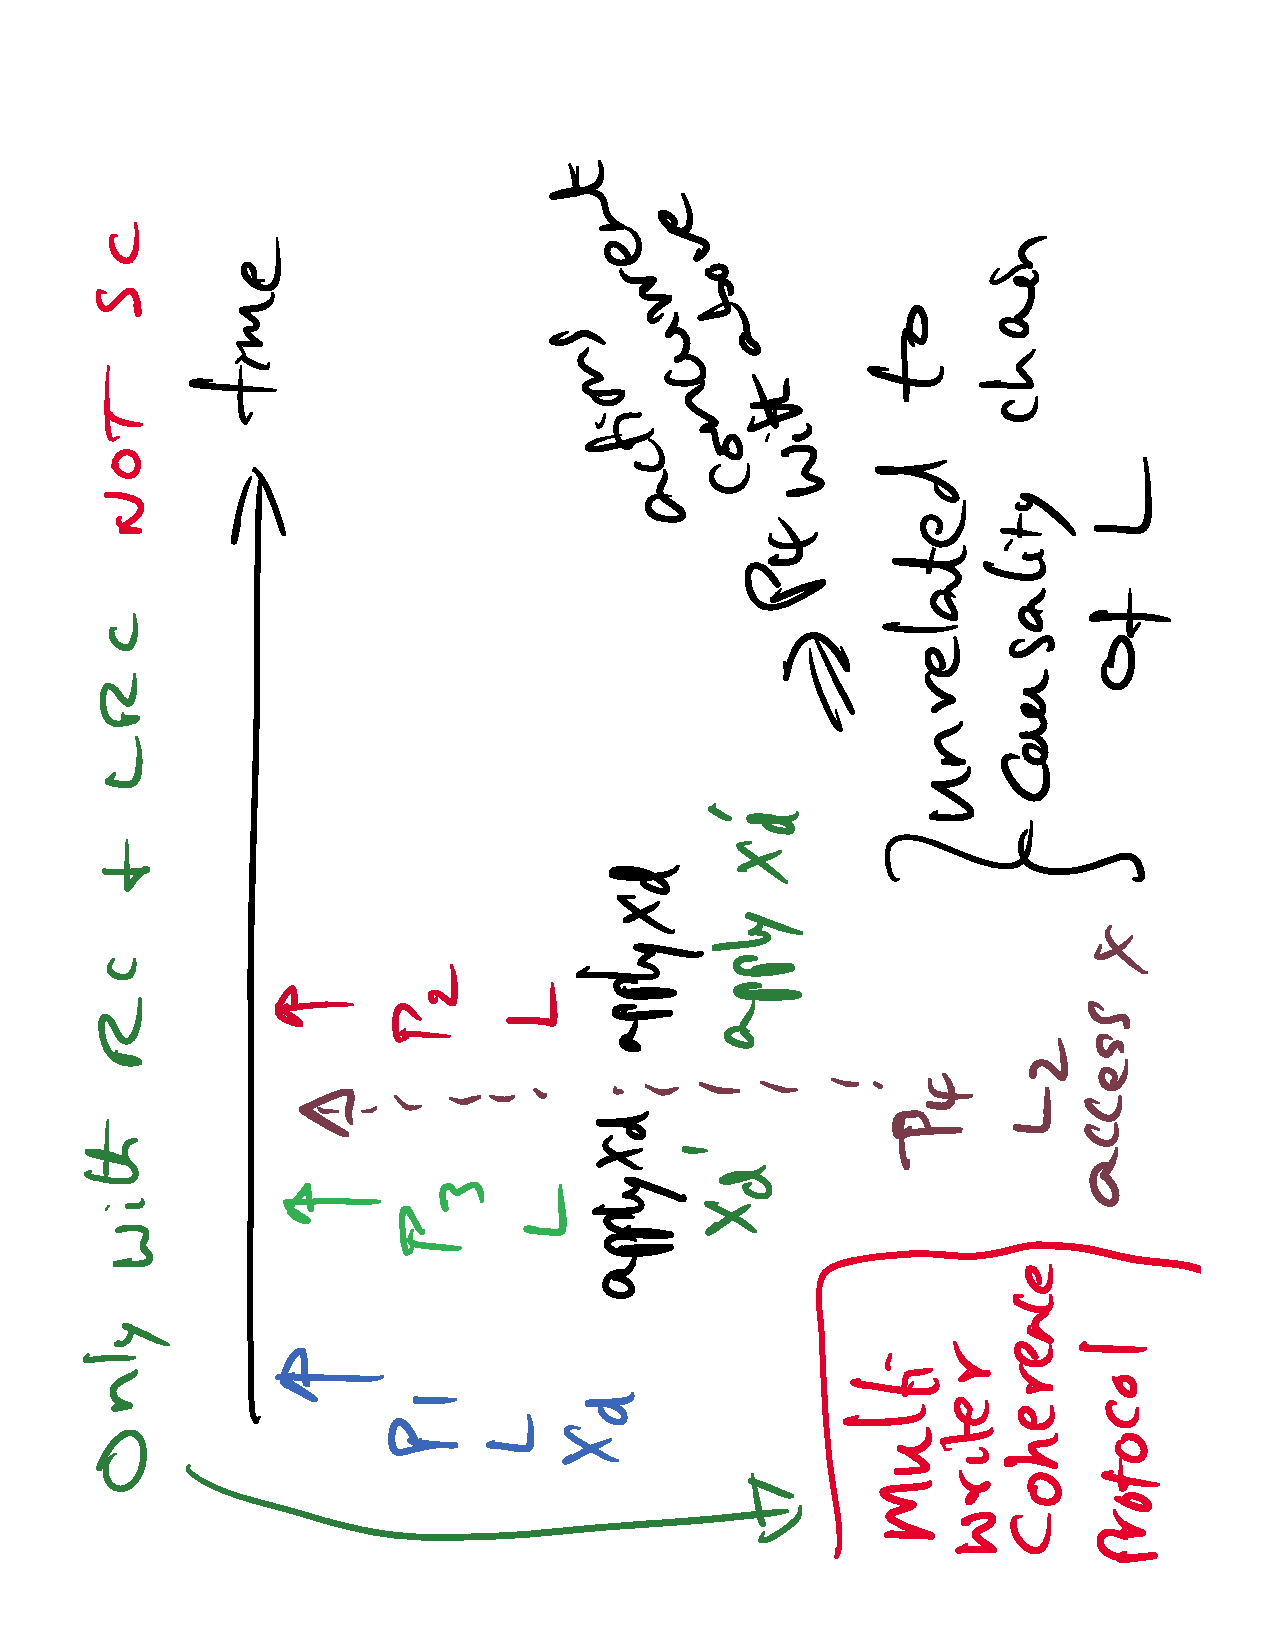
\includegraphics[width=\fullsize, angle=-90]{Figures/example-mwcp}
\caption{An example of multiple-writer case.}\label{fig: mwcp-example}
\end{figure}

Now, it is the time to talk about the multiple-writer part of it. Note that, it could be multiple user 
data structures present in a given page {\code x}. If that is the case, the programmer probably 
has different locks for accessing different portions of the data structures that happened to all 
fit within this page {\code x}. So it is conceivable that when all of the processes shown 
in~\autoref{fig: mwcp-example} were going on. Another processor, say $P4$, and a thread that was running on processor 
$P4$ got a completely different lock, say {\code L'}. And it is accessing some data structure 
that happens to be in the same page {\code x}. This is perfectly fine. The DSM software is 
not going to do anything in terms of the ``diffs'' that is has created with respect to the 
page {\code x} because of lock {\code L}. That is completely different set of actions compared to a different 
lock acquisition, say {\code L'}. So if in fact that other thread that is running on $P4$ 
got executed and modified {\code x}. When $P2$ gets its lock {\code L}, the DSM 
software is going to bring the ``diffs'' only from the previous holders of {\bf the same lock}. 
$P4$ was not using {\code L}, instead it was using {\code L'}, even though it accessed the same page 
and modified a different portion of that page. The DSM software is going to assume 
that changes made by $P4$ to {\code x} is irrelevant as far as $P2$'s critical section is concerned. 
So that is the important thing, that is where the multiple-writer coherence protocol semantic comes 
in. That simultaneously the same page could be modified by several different threads on several different 
processors. 


\begin{figure}
\centering
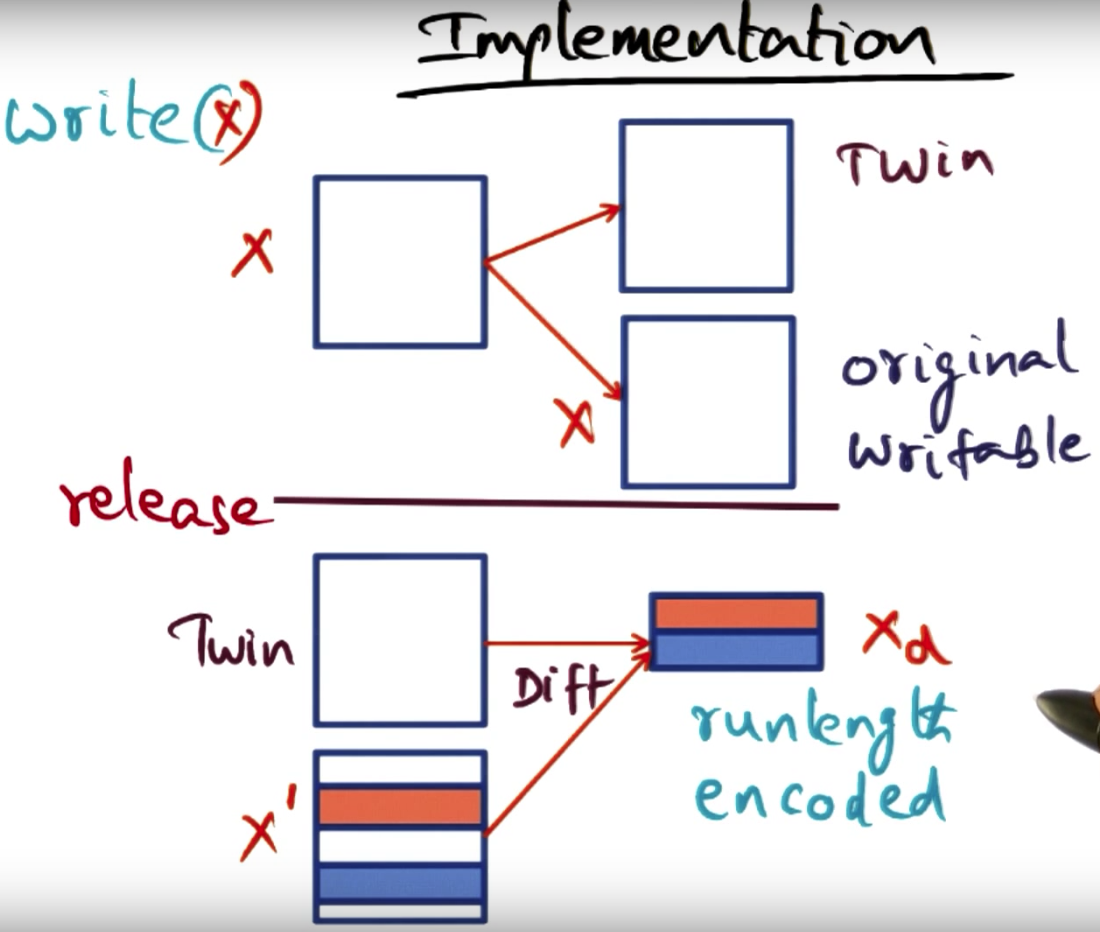
\includegraphics[width=\fullsize]{Figures/impl}
\caption{Implementation.}\label{fig: impl}
\end{figure}

\noindent
{\bf Implementation.} Now, let us look at some implementation details. What is going to happen is 
when a process or a thread on a processor tries to write to a page {\code x}. At the point of 
writing to that page {\code x}, the operating system will make a ``twin'' for this page {\code x}, so 
there is the original page and the ``twin'' for this page. And the original page is writable by 
this processor of which mapping is there in the page table. This new copy, {\it i.e.,} the ``twin'', 
has been created in physical memory, is not mapped in the page table of any process. It is just an additional 
copy of the same page created by the operating system as a twin. When the thread reaches the release point, 
as mentioned in previous lecture, what the DSM software is going to do, is to compute the ``diffs'' between 
the changes that have been made, and the original version. Note that, here by ``original version'', we 
mean the twin of the page {\code x}. And the ``diffs'' is going to be computed as a run-length encoded~\cite{rle} ``diffs'', 
meaning that all of the page has not been modified, as shown in~\autoref{fig: impl}, only the colored portions are being 
modified, so the ``diffs'' is going to be computed as the colored parts. The ``diffs'' is a data structure 
that has been created by the DSM software to remember the changes that have been made to this page {\code x} 
prior to the release. As you might have been imagined already, when the same lock that governs accesses to this 
page which was release at the ``release line'' in~\autoref{fig: impl}, is acquired by a different processor. 
At the point of acquisition, what we are going to do is we are going to invalidate all the pages that 
were touched in the critical section including {\code x}. So {\code x} will be invalidated 
at the point of acquisition of the same lock that is governing this critical section. When that 
processor has a page fault for page {\code x}, the DSM software knows it has to get the ``diffs'' together with 
the original copy of this page in order to update the page and give it to the current lock acquirer. So that 
is what goes on under the covers. Note that, once the thread has completed its release operation, we will 
write protect the page {\code x} to indicate that that thread cannot modify this page anymore unless 
it gets in the critical section and we have to do the coherence actions again. And that is the implementation 
of the protocol. And once we write protect the page {\code x}, we can get rid of the ``twin''. The use of this 
twin is complete we only need it in order to compute the ``diffs''. We have computed it and we write protected 
original page and everything that needs to be done. Getting rid of the ``twin'' essentially means that we are 
freeing up the physical memory that we allocated for creating the ``twin'' in the first place. 

As mentioned earlier, it is a multiple-writer protocol. Therefore, the action shown in~\autoref{fig: impl} can be happening 
simultaneously for the same page {\code x} on different nodes of the cluster. If multiple writes happen to 
the same portion of the same page under different lock, which will result in {\bf data race}. However that is 
the user's problem. That is not the problem of the DSM software. It is an application problem, because it represents 
a data race that should not been there if the application was constructed correctly. So this implementation 
that detailed above is an example of the cooperation between the DSM software and the operating system. 
In particular, TreadMarks~\cite{Amza1996DSM} implemented this LRC multiple-writer coherence protocol 
on a UNIX system. And in the UNIX system, the operating system generates an exception called {\bf SIGSEGV} in the 
operating system layer when a shared page is accessed by a thread. This exception is caught by the 
thread library's runtime handler and at that time the DSM software gets into gear, contacts the owner of the page, 
checks the status of the page. And if the page in invalid then it gets the page and 
the ``diffs'' for that page. Once it brings in the contents of the page and the ``diffs'', it creates a current 
version of the page. And if the processor that is trying to access the page is making a read access, then 
there is no problem. But if the process that wants to write to the page, then it creates a ``twin'' and does 
all the things that mentioned above. So one thing that you will notice is that there is space overhead for the 
creation of the ``twin'' at the point of the write, and the ``diffs'' at the point of release. As time goes by, 
there could be a lot of these ``diffs''\footnote{Note that, the ``twin'' can be got rid of at the point of release.}. 
Imagine that a page was touched by ten different processors. In that case, there are going to be ``diffs'' 
lying on ten different processors. And if an eleven processor wants to access the same page, the DSM software 
has to go and bring all the ``diffs'' from the ten prior ``users'' of the page, get the original page from 
the owner, apply the ``diffs'' to create the new page. A lot of latency is involved before the processor who 
nees the page can start using it. Besides that there are a lot of space overhead noticing that 
all these ``diffs'' lying around. So one of the things that happens in the DSM software is garbage collection. 
That is, you keep a watermark of what is the amount of ``diffs'' that have been created in the 
entire system. If it exceeds a threshold, then you start applying these ``diffs'' to the original copy 
of the page, at the owner. So that you can then get rid of these ``diffs'' completely. You do not want to 
do this too eagerly, and you do not want wait for too long also, because if a page has not been accessed 
for a long time, ``diffs'' are going to be lying around for a long time. So there will be a demon process 
in every node that every once a while wakes up and sees how much ``diffs'' have been created in my node. If it exceeds 
the threshold then it will apply these ``diffs'' to the original copy of the page. 

\section{Non-Page-based DSM}\label{sec: np-dsm}

In this lecture, we have covered distributed shared memory systems. In particular, a distributed shared 
memory system called TreadMarks~\cite{Amza1996DSM} that uses lazy release consistency and multiple-writer 
coherence protocol, was detailed. 
Now let us get some thought of non-page based distributed shared memory systems. There have been systems 
that have been built that do not have the granularity of a page for coherence maintenance. As mentioned 
earlier, if you want to maintain granularity not at the page level, then you have to track individual 
reads and writes that is happening on a thread. 

\noindent
{\bf Library based DSM.} One approach is called a {\bf library based } approach. The idea is as follows. 
The programming library is going to give you a way by which you can annotate shared variables that 
you are going to use in your program. Whenever you touch a shared variable. Part of creating the executable 
is to cause a trap at the point of access to the shared variable. So that the DSM software will be 
contacted, and it can then take coherence actions at the point of access to the shared variables. 
So in this case, there is no operating system support needed because in the binary itself, we are 
making sure that at the point of access, we are going to result in a trap that will get us into the trap handler 
that is part of the DSM software. So that it can take the coherence actions. And examples of 
systems that use this mechanism include Shasta~\cite{shasta}, that was done at Digital Equipment 
Corporation, and Beehive~\cite{beehive}, which was done at Georgia Tech. And because we are doing this sharing 
at the level of variables, you do not have any false sharing which is possible with page based 
systems and single writer cache coherence protocol. Once the DSM software takes the coherence actions, which might 
include fetching the data that is associated with the variables you are trying to access, then 
DSm software can resume this thread that caused the trap in the first place.

\noindent
{\bf Structured DSM.} Another approach to providing the shared abstraction is not at the level of 
memory locations, but at the level of structures that are meaningful for an application. 
And that is what is called {\bf structured DSM}. The idea is as follows. There is a programming library 
which actually provides abstraction that can be manipulated in an application program. And 
the abstractions can be manipulated using API calls, that are part of the language runtime. 
So when the application makes the API call, the language runtime gets into gear and asks what coherence actions 
are needed to make in order to satisfy this API call. All of those coherence actions are 
going to be taken at the point of that API call, and that might include fetching data from a remote 
node in the cluster. And once the semantics of the API call have been executed by the language runtime, 
then it is going to resume this thread that made the call in the first place. Again, there is not operating 
system support for this. And the structured DSM is a very popular approach that has been used 
in systems such as Linda~\cite{linda}, Orca~\cite{bal1992orca}, and Stampede~\cite{nikhil1998stampede} that was 
done at Georgia Tech., and successors to Stampede called Stampede RT~\cite{stampedert} and 
PTS (In the later-on lectures of this course, we will see PTS as an example of a structured DSM system)~\cite{Hilley2000PTS}. 

\section{DSM and Speedup}\label{sec: permance}

\begin{figure}[!htb]
\centering
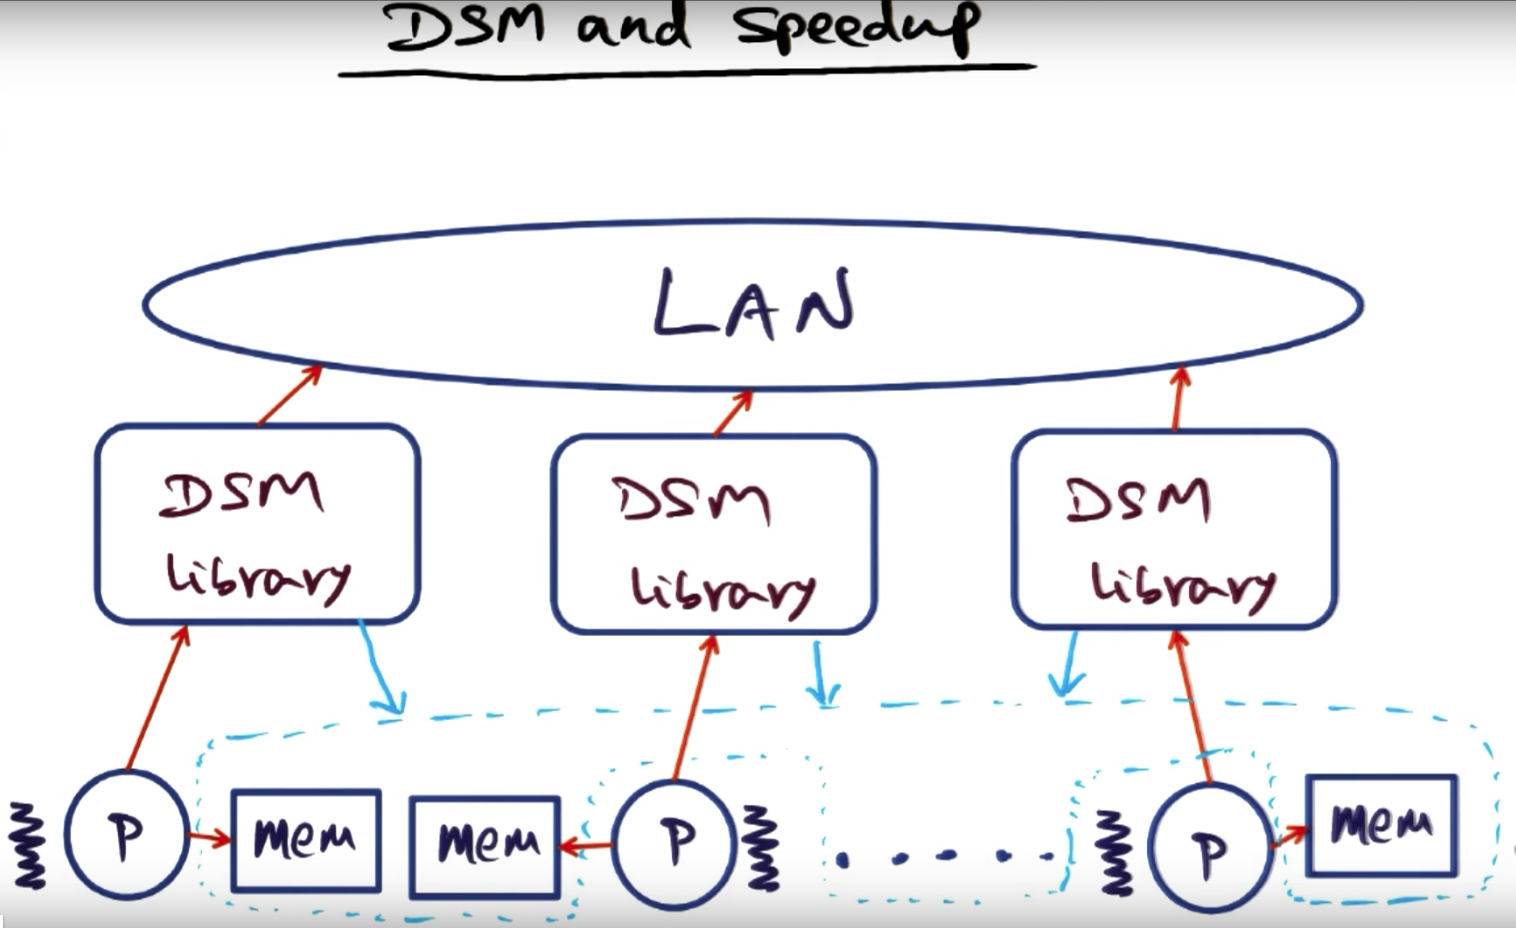
\includegraphics[width=\fullsize]{Figures/performance.PNG}
\caption{DSM and speedup.}\label{fig: speedup}
\end{figure}

As shown in~\autoref{fig: speedup}, we have an illusion of shared memory, which is implemented by physical memories 
that strewn all over the entire cluster. And the hope is that the application that is running on 
the different nodes of this cluster will actually get speedup with increasing number of 
processes, but such speedup is not automatic if the sharing that we are doing. Even though 
DSM gives you the ability to share memory across the network, recall what our good friend Chuck 
Thacker told us, {\it shared memory scales really well when you do not share memory.} So if the sharing is 
to fine-grain, then no hope of speedup, especially with DSM system because it was only an illusion of 
shared memory via software not even physical shared memory. Even physically shared memory can lead to 
overheads. So this illusion through software can result in even more overheads, so we should 
be even more careful on how you share and what we share. So the basic principle is that the computation to the 
communication ratio has to be very high if you want any hope of speedup. In other words, 
the critical sections that are executed to modify data structures better be really really 
hefty critical structures before somebody else needs to access the same portion of the data. 
So what does this mean for shared memory codes basically is that if the code has a lot of 
dynamic data structures that are manipulated with pointer then it can lead to a lot of implicit 
communication across the local area network. That is the bane of distributed shared memory that 
pointer codes may result in increasing overhead for coherence maintenance. So we have to be 
extreme careful on how to structure codes that can execute efficiently on distributed shared memory systems. 




\bibliographystyle{IEEEtran}
\bibliography{references}


\end{document}
